% !TeX root = Project.tex
\subsection{The Definition of the Riemann Integral}
The definition of the Riemann integral involves a few steps, and so it's going to take a little patience. The first step is defining a step function (no pun intended).
%
\begin{figure}[h]
	\centering
	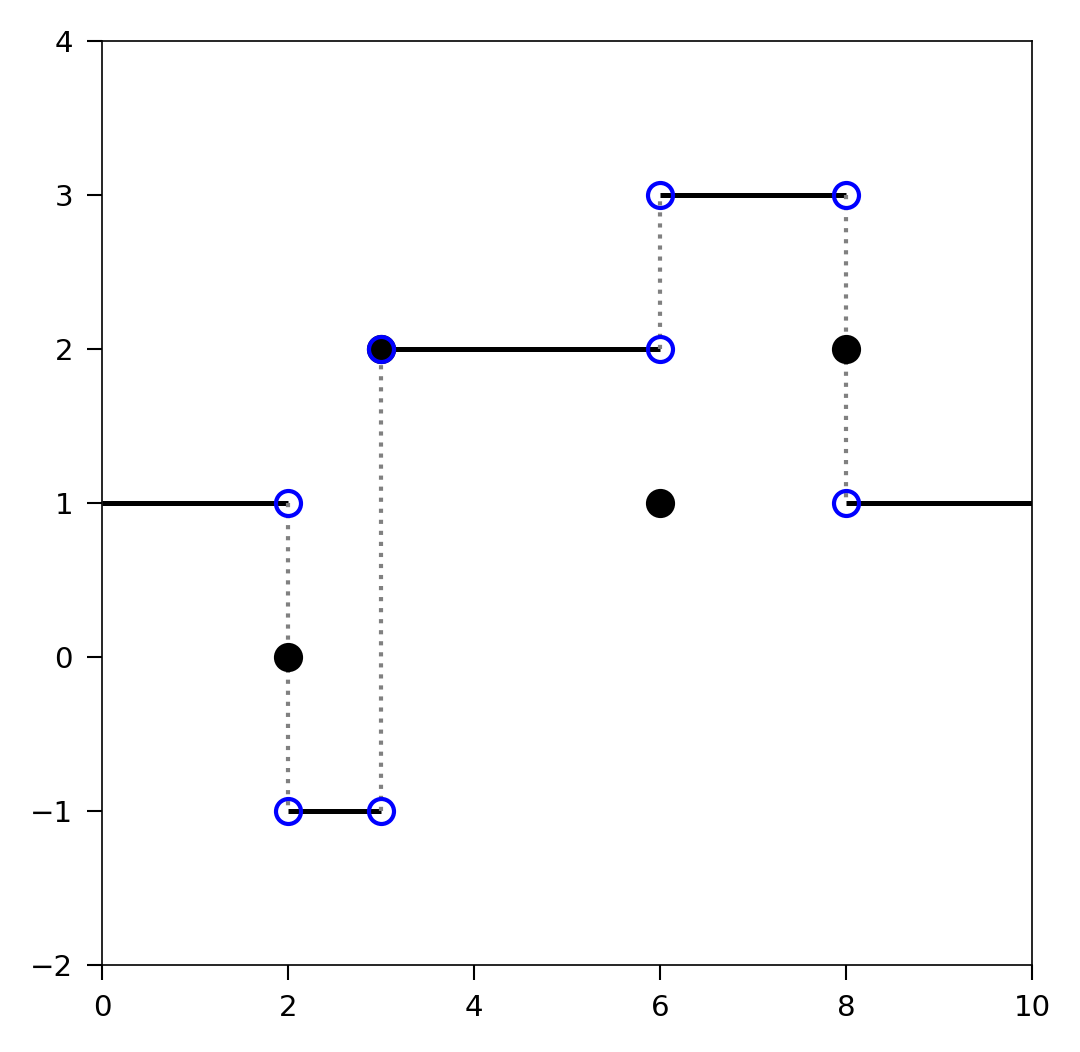
\includegraphics{Code/Step.png}
	\caption{A Step Function}
	\label{fig:step}
\end{figure}

A function is called a step function if and only if there exists some finite sequence of points such that the function is constant between any two adjacent points. So, for the function with the graph shown below in Figure \ref{fig:step}, the points $\{0, 2, 3, 6, 8, 10\}$ are the finite sequence which make this a step function. We will often index the elements of sequence using $n$, and label each element $x_n$. We can call sequence this a \emph{`representation'} of the function, and we can call the sequence of constant heights just \emph{before} each point the corresponding \emph{`height sequence'}. The \emph{height sequence} along with the representation fully describe the function.

\medskip
Note two important points;
\begin{itemize}
	\item We could have picked $\{0, 1, 2, 3, 4, 5, 6, 7, 8, 9, 10\}$ to be our representation, since the function also happens to constant between any two adjacent integers. 
	\item It doesn't really matter what the function is {\em at} the points $x_n$ --- we only care whether the function is constant {\em between} the points. In our graph, 2, 3, 6, and 8 are discontinues, but that doesn't matter since they're also in our sequence of points. 
\end{itemize}

The formal definition is as follows;
\begin{definition}[Step Function]
    $\phi\colon \ [a, b] \rightarrow \R$ is a {\em step function}
    \begin{itemize}
        \item[$\logeq$]
            $\phi \in \mathcal{S}([a, b])$
        \item[$\logeq$]
            $\exists N \! \in \! \N$ \ and \ $\exists X = (x_n)_{n=0}^N$ : $a = x_0 < x_1 < \ldots < x_{n-1} < x_n = b$, \ and \ $\forall m\in\N_{< N}$ we have $\exists! c_m \in \R$ : $\forall z \in (x_{m-1}, x_{m})$ we have $\phi(z) = c_m$.
    \end{itemize}
\end{definition}

This also defines \emph{the set of all step functions on} $[a, b]$ as $\mathcal{S}[a, b]$. This kind of thing is done a lot in analysis --- we often want to look at the set of all things which satisfy some property. We normally don't have to \emph{find} them all --- we just need a way to represent the full set. The fact that it'd be near impossible to try to imagine the set $\mathcal{S}([a, b])$ is irrelevant --- it's just important we know it exists.

\medskip
Next, we want to define what it means to integrate a step function. Remember, the point of working with step functions is because it's easy to find the area of rectangles, and integration is all about finding areas. So where are the rectangles? 

\medskip
As is hinted at by Figure \ref{fig:step}, we can make the bases of the rectangles the width the intervals $(x_{n-1}, x_n)$, and the heights the constant $c$ which values in this interval take. This is made even clearer by Figure \ref{fig:stepfilled}, where we can also see that the sometimes our heights will have negative values, and that's okay --- these areas are just taken away from the total area instead of added to it.
 
What's not okay is that any one step function may have different sequences which we can use to prove that it's a step function --- or in other words, the same step function may have different but equally valid representations. We defined the integral of a step function in terms it's representation, but how do we know that different representations of the same function produce the same integral? Figure \ref{fig:stepfilled} demonstrates that, given the representations $\{0, 2, 3, 6, 8, 10\}$ and $\{0, 1, 2, \ldots, 10\}$ of \ref{fig:step}, we're fine, and the areas are equal. It turns out that this is the case in general --- the integral of a step function is independent of the chosen representation.

\begin{figure}[h]
  \centering
  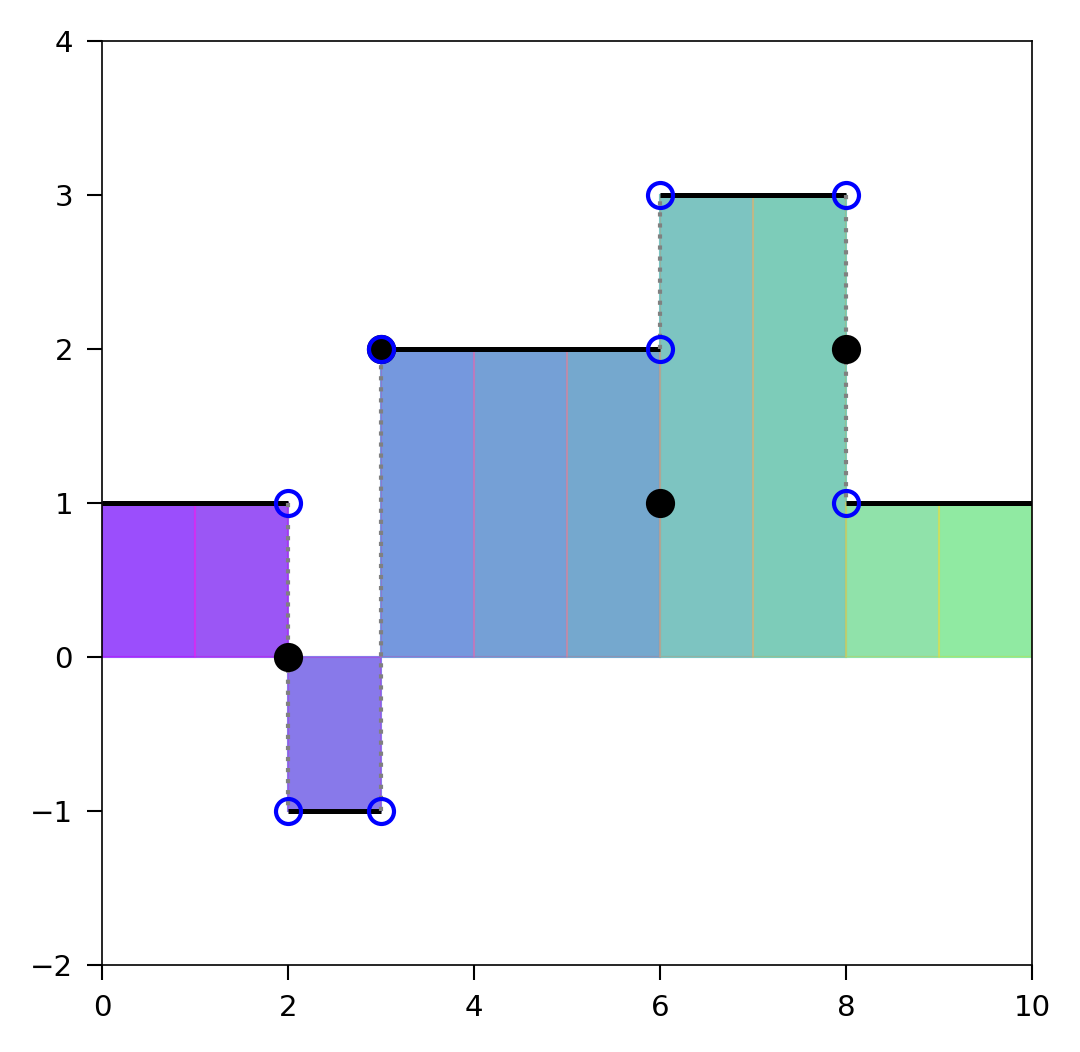
\includegraphics{Code/StepFilled2.png}
  \captionof{figure}{Integral of \ref{fig:step}}
  \label{fig:stepfilled}
\end{figure}

\begin{definition}[Integral of a Step Function]
\label{def:stepint}
	Given
	\begin{itemize}
	\item 
		$\phi \in \mathcal{S}([a, b])$,
	\item
		$N \in \N$ and the representation $(x_n)_{n=0}^N$ of $\phi$,
	\item
		the corresponding \emph{height sequence} $(c_n)_{n=1}^N : \phi(x) = c_n \quad \forall x \in (x_{n-1}, x_{n})$,
	\end{itemize}
	then the \emph{Integral} of $\phi$ as a function of $x$ on $[a, b]$ is
	\begin{equation}
	\begin{split}
		&\intx{\phi(x)} \\
		\defeq \quad &\sum_{i=1}^N c_i(x_{i} - x_{i-1}).
	\end{split}
	\end{equation}
\end{definition}%

To show that the integral is independent of the choice of representation, we'd need to show that if we had two arbitrary representations $(x_n)_{n=0}^N$ and $(x'_m)_{m=0}^M$ with \emph{height sequences} $(c_n)_{n=1}^N$ and $(c'_m)_{m=1}^M$ resp. then $$\sum_{i=1}^N c_i(x_{i} - x_{i-1}) = \sum_{j=1}^M c'_j(x'_{j} - x'_{j-1})$$. 
The idea behind why this is true is the following; 
\begin{itemize}
\renewcommand\labelitemi{$\times$}
\item
Assuming first that one seqence is a subseqence of the other, we will focus on the representation that is more `fine' --- i.e. the one that has smaller width rectangles; ones which are divisions of the rectangles in the `coarser' representation. 
\item
We look at it in sections; with the sections being the steps of the coarser representation. So, in \ref{fig:step}, we'd look at $\{0, 1, 2 \ldots, 10\}$ between 0 and 2, then 2 and 3, then 3 and 6 $\ldots$ etc. 
\item
The two representations are for a single the step function, and we use this group adjacent rectangles with the same height. $\phi(x)$ must be constant in the section we are looking at, and so we know that all the rectangles here have the same height
\item
Then we can use the distributive property of multiplication to view the smaller width rectangles of the same height as one big rectangle with the width of the whole section. And boom, we're done, since those big rectangles are exactly the ones which you would use when integrating using the coarser representation.
\item[$\otimes$]
If neither representation is contained within the other, then we can just create a third representation which is the union the first ones. Both original sequences will be coarser than this new one, and so we can use the same reasoning as before, plus transitivity and symmetry, to prove the integrals are the same.
\end{itemize}

\begin{figure}[t] % Remember to change this to 'h'!
	\renewcommand{\subfigcapskip}{-5pt}
	\centering
	\subfigure[Focus on finer representation.]{%
		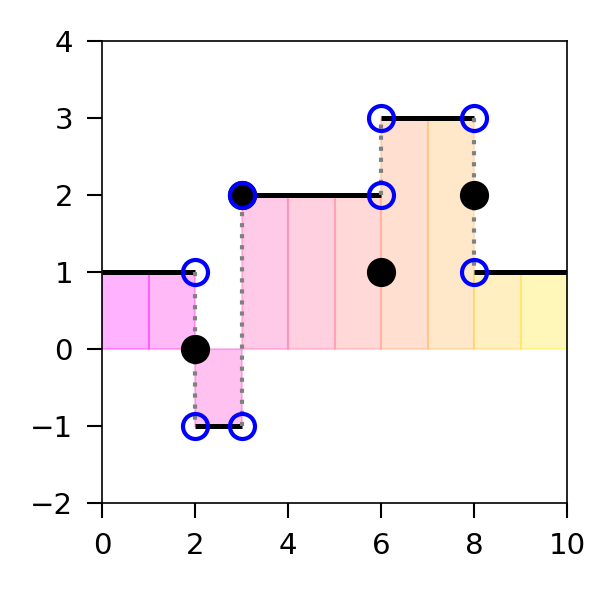
\includegraphics{Code/StepFilledSmall.png}}\qquad
	\subfigure[Look at section between 3 and 6.]{%
		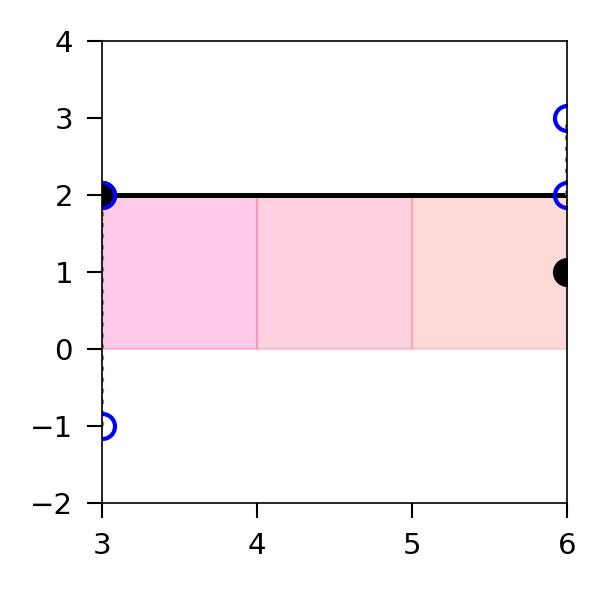
\includegraphics{Code/StepFilledFocused.png}}\\
	\subfigure[Group rectangles.]{%
		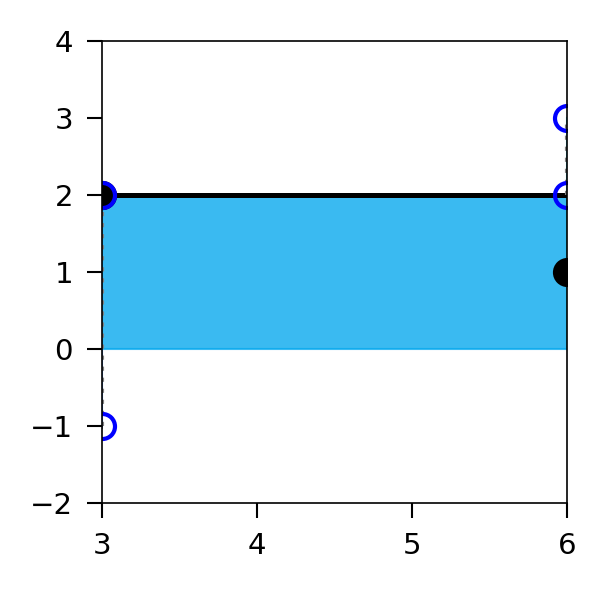
\includegraphics{Code/StepFilledFocused3.png}}\qquad
	\subfigure[\bf Boom]{%
		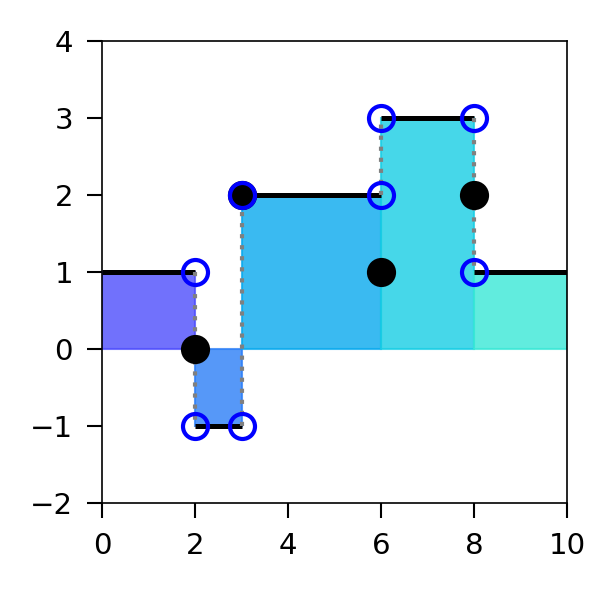
\includegraphics{Code/StepFilled3Small.png}}
	\caption{Different representations of the same function.}
	\label{fig:representations}
\end{figure}

\begin{prop}
	Given,
	\begin{itemize}
		\item
		$\phi \in \allstep$,
		\item
		$N, M [=N'] \in \N$ and the representations $(x_n)_{n=0}^N$ and $(x'_{m [=n']})_{m=0}^M$ of $\phi$,
		\item
		The respective height sequences $(c_n)_{n=1}^N$ and $(c'_m)_{m=1}^M$ of these representations,
	\end{itemize}
	then
	\begin{equation}
	\sum_{i=1}^N c_i(x_{i} - x_{i-1}) = \sum_{j=1}^M c'_j(x'_{j} - x'_{j-1}).
	\end{equation}
\end{prop}
\begin{cproof} 
	\leavevmode \\
	\emph{Case 1:} $\{x_n; n \in \N_{n<N}\} \subset \{x'_m; m \in \N_{m<M}\}$:
	\begin{IEEEeqnarray}{rCl}
		&  & \{x_n; n \in \N_{<N}\} \subset \{x'_m; m \in \N_{<M}\} \nonumber \\
		& \Leftrightarrow \quad & \exists J = (j_n)_{n=0}^N \nonumber \\
		&  & : 0 = j_0 < j_1 < \ldots < j_{n-1} < j_n = m \text{ and } k \in \N_{<N} \text{ we have } x_k = x'_{j_k} \nonumber
	\end{IEEEeqnarray}
	Hence,
	\begin{IEEEeqnarray}{rCl}
	\sum_{j=1}^M  c'_j(x'_{j} - x'_{j-1})  & = & \sum_{k=0}^N \; \sum_{j = j_{k-1}}^{j_k} \!\! c'_j(x'_{j} - x'_{j-1}) \nonumber \\
	& = & \sum_{k=0}^N \; c'_{j_k} \!\!\! \sum_{j = j_{k-1}}^{j_k} \!\! (x'_{j} - x'_{j-1}) \nonumber \\
	& = & \sum_{k=1}^N  c_k(x_{k} - x_{k-1}) \nonumber 
	\end{IEEEeqnarray}
	\emph{Case 2:} Arbitrary representations $X = \{x_n; n \in \N_{<N}\} \text{ and } X' = \{x'_{n'}; n' \in \N_{<N'}\}$:

	\medskip
	Let $X'' = \{x''_{n''}; x"_{n''} \in X\cup X'\}$.
	\begin{IEEEeqnarray}{rCc}
		&  & \{x_n; n \in \N_{n<N}\} \subset \{x''_{n''}; n'' \in \N_{<N''}\} \supset \{x'_{n'}; n' \in \N_{m<M}\} \vspace{3pt}\nonumber \\
		& \Rightarrow \quad & \sum_{X} = \sum_{X''} = \sum_{X'} \nonumber 
	\end{IEEEeqnarray}
\end{cproof}
Now we are ready to define the \emph{Riemann Intergral} of any function $f\colon [a, b] \rightarrow \R$ $\ldots$ almost. We first need to define 2 seperate upper and lower intergrals, and then if they are the same, what we call that the {Reimann Intergral} of the function. This is actually why $\mathbbm{1}_\Q(x)$ is not \emph{Reimann Integrable}; it's upper and lower intergrals do not coincide. 

\medskip
To find the \emph{Upper Reimann Intergral} of $f$, first find \emph{all} the step functions which bound it from above, then calculate their integrals using \dref{def:stepint} and then, finally, define the smallest of these intergrals to be the \emph{Upper Reimann Intergral.} To find the \emph{Lower Reimann Integral,} you do the same thing, but from below. The set of Reimann Integrable functios on $[a,b]$ is $\mathcal{R}([a, b])$.

\medskip
Figure \ref{fig:areaapprox} tries to illustrate this, but it's important to remember that we aren't looking at a seqence of step functions, we are looking at \emph{all of them}. How to calculate/approximate intergrals using step functions is a whole thing in itself --- I wish I had started writing this sooner so that I could get into it because it's super interesting, but alas. Anyway, now we can define \emph{Reimann Integration} for real:

\begin{definition}[Riemann Intergration]
	Given  
	\begin{itemize}
	\item
		$f\colon [a, b] \rightarrow \R$,
	\item
		$S_l \subset \allstep : \psi \in S_l \Leftrightarrow \ \psi(x) \leq f(x) \quad \forall x \in [a, b] $,
	\item
		$S_u \subset \allstep : \phi \in S_u \Leftrightarrow \ \phi(x) \geq f(x') \quad \forall x' \in [a, b] $,
	\end{itemize}
	then the \emph{Lower Riemann Integral} of $f$ is
	\begin{equation}
		\underline {\int} \, f(x) \, dx \defeq \sup \left\{\intx{\psi(x)}; \;\; \psi \in S_l\right\}
		\label{eq:lowerriemann}
	\end{equation} 
	and the \emph{Upper Reimann Integral} is
	\begin{equation}
		\overline {\int} \, f(x) \, dx \defeq \inf \left\{\intx{\phi(x)}; \;\; \phi \in S_u\right\}.
		\label{eq:upperriemann}
	\end{equation}
	If \eqref{eq:lowerriemann} = \eqref{eq:upperriemann}, then $f$ is \emph{Reimann Integrable} the \emph{Reimann Integral} of $f$ as a function of $x$ is 
	\begin{equation}
		\intx{f(x)} \defeq \underline {\int} \, f(x) \, dx = \overline {\int} \, f(x) \, dx
	\end{equation}
\end{definition}